\chapter{A velocidade das reações}\label{ch:g12:reaction-rates}

Uma garrafa de leite esquecida em cima da pia azeda em uns dois dias; na
geladeira, ela dura mais de uma semana. Um fogo de artifício \omterm{def:g4:what-a-fire-needs:burning}{queima} numa
fração de segundo, enquanto uma estátua de calcário num parque da cidade
se desgasta ao longo de séculos. As \omterm{def:g8:balanced-equations:equation}{equações balanceadas} e as \omterm{def:g10:reaction-progress-table:extent}{tabelas de
avanço} dizem o que uma reação dá e quanto; elas não dizem nada sobre a
rapidez. Este capítulo mede a velocidade das reações, descobre o que a
controla e descreve a maneira mais simples de uma reação ir ficando mais
lenta à medida que avança.

\begin{recall}
A concentração de uma solução (\cref{ch:g10:concentration-and-dilution})
e o avanço de uma reação (\cref{ch:g10:reaction-progress-table}). A
\omterm{def:g11:absorbance:absorbance}{absorbância} de uma solução diluída é proporcional à concentração da
espécie colorida (\cref{ch:g11:absorbance}). Uma \omterm{def:g11:titration:titration}{titulação} mede a
\omterm{def:g10:the-mole:amount}{quantidade de matéria} de uma espécie (\cref{ch:g11:titration}).
\end{recall}

\begin{omfigure}
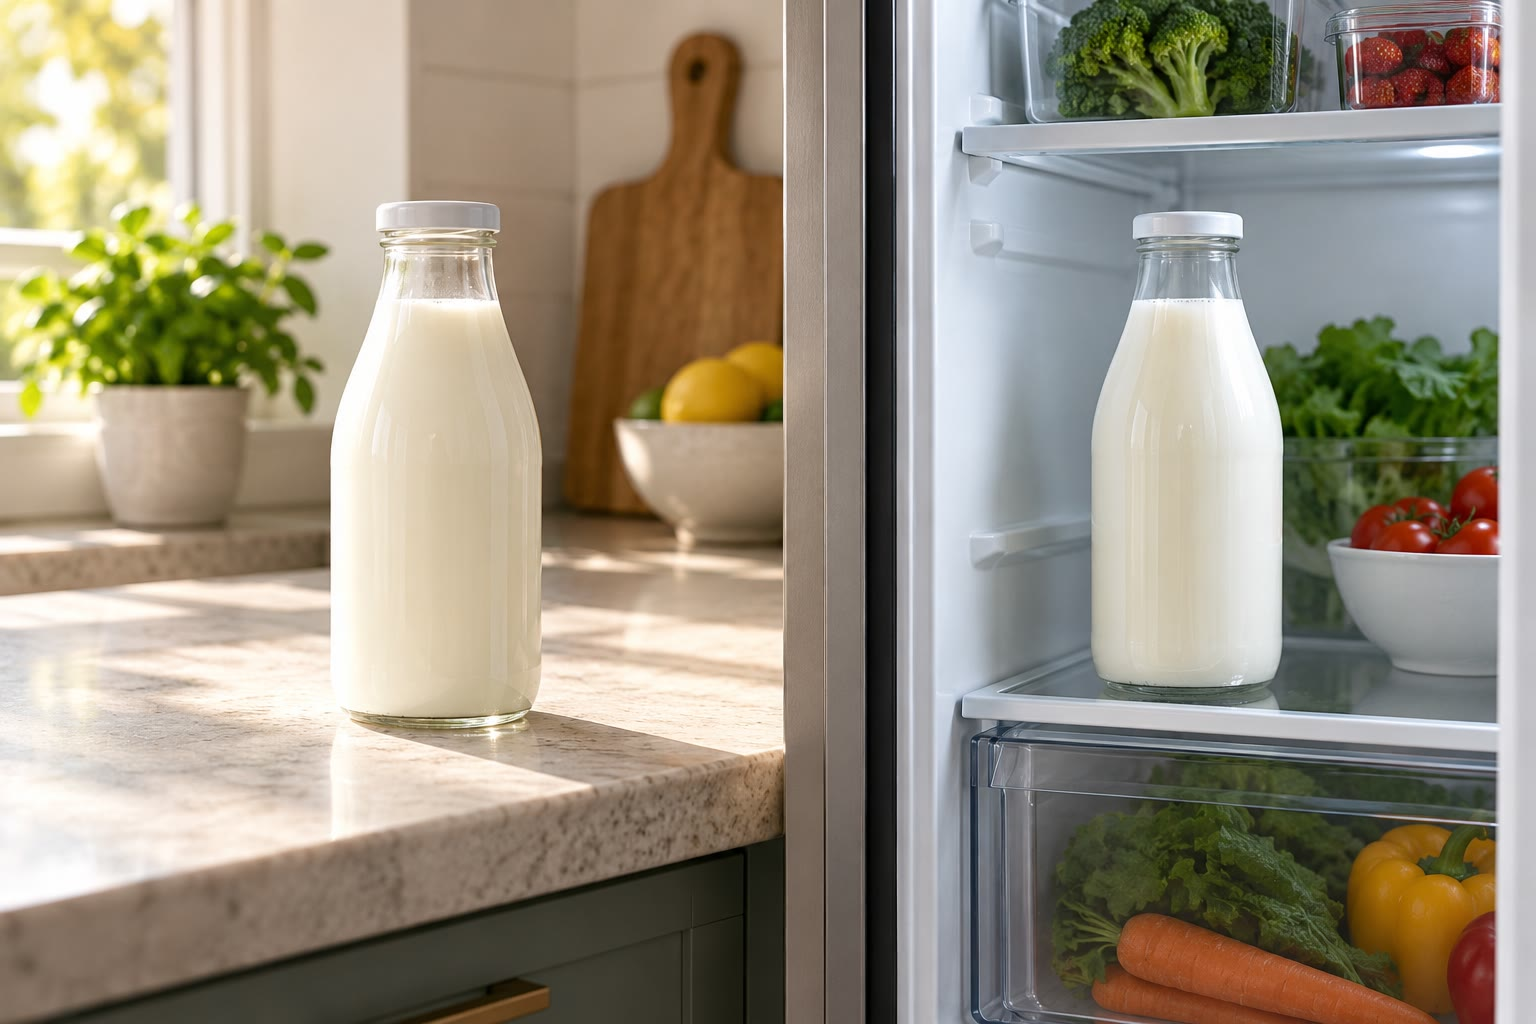
\includegraphics[width=0.48\linewidth]{images/book1/ai/g12-milk-counter-fridge.jpg}

{\small O mesmo leite, em cima da pia e na geladeira: as reações que o
azedam são mais lentas no frio.}
\end{omfigure}

\section{Acompanhar uma reação no tempo}

Algumas reações terminam assim que os \omterm{def:g7:chemical-reactions:reactant}{reagentes} se encontram: a
\omterm{def:g9:ions:precipitate}{precipitação} do cloreto de prata, a reação de um ácido com uma base.
Outras levam minutos, horas ou anos. Para estudar uma reação lenta, os
químicos medem a concentração de um \omterm{def:g7:chemical-reactions:reactant}{reagente} ou de um produto em
intervalos regulares. Eles podem
\begin{itemize}
  \item retirar pequenas amostras, interromper a reação em cada uma e
        titulá-las;
  \item medir a \omterm{def:g11:absorbance:absorbance}{absorbância} da solução, quando um \omterm{def:g7:chemical-reactions:reactant}{reagente} ou um produto
        é colorido;
  \item medir a pressão ou o volume de um gás liberado, ou a
        condutividade de uma solução cujos \omterm{def:g9:ions:ion}{íons} mudam.
\end{itemize}

\begin{definition}[Interrupção da reação]\label{def:g12:reaction-rates:quenching}
A \emph{interrupção da reação}\index{interrupcao da reacao@interrupção da reação} numa amostra
consiste em parar a reação nela, ou torná-la muito mais lenta, no
momento em que a amostra é retirada, em geral resfriando-a de repente e
diluindo-a, de modo que a sua composição possa ser medida com calma.
\end{definition}

\begin{inthelab}[Interromper a reação numa amostra]
A cada cinco minutos, \qty{10.0}{mL} da \omterm{def:g6:pure-substances-and-mixtures:mixture}{mistura} reacional são retirados
com uma pipeta e despejados num béquer com cerca de \qty{40}{mL} de água
gelada. Diluída cinco vezes e resfriada perto de \qty{0}{\celsius}, a
reação fica tão lenta que pode ser considerada parada; a amostra é então
titulada. O instante da amostra é o momento em que ela foi despejada na
água gelada, não o momento da \omterm{def:g11:titration:titration}{titulação}.
\end{inthelab}

\begin{omfigure}
\begin{tikzpicture}[font=\small, scale=0.8]
  \pic[transform shape] at (0,0) {erlenmeyer={0.4}{orange!25}};
  \node[anchor=north, align=center] at (0,-0.15) {mistura\\ reacional};
  \pic[transform shape, rotate=-35] at (1.4,1.2) {pipette={0.6}{orange!25}};
  \draw[omProp, very thick, -{Stealth}] (1.6,0.8) -- (2.9,0.8);
  \node[anchor=south] at (2.25,0.85) {\qty{10.0}{mL}};
  \pic[transform shape] at (4,0) {beaker={0.55}{cyan!12}};
  \foreach \p in {(3.6,0.4),(4.2,0.6),(3.9,0.85),(4.4,0.3)}
    \draw[black!30, fill=white] \p ++(-0.1,-0.08) rectangle ++(0.2,0.16);
  \node[anchor=north, align=center] at (4,-0.15) {água gelada:\\ reação parada};
  \draw[omProp, very thick, -{Stealth}] (5.1,0.8) -- (6.4,0.8);
  \pic[transform shape] at (7.5,0) {erlenmeyer={0.35}{orange!12}};
  \pic[transform shape] at (7.5,2.75) {burette={0.7}{violet!45}};
  \node[anchor=north, align=center] at (7.5,-0.15) {titulação\\ da amostra};
\end{tikzpicture}

{\small Acompanhar uma reação por amostragem: retirar uma amostra,
interromper a reação nela e depois medi-la com calma.}
\end{omfigure}

\section{Os fatores cinéticos}

\begin{definition}[Fator cinético]\label{def:g12:reaction-rates:kinetic-factor}
Um \emph{fator cinético}\index{fator cinetico@fator cinético} é uma grandeza que muda a
velocidade de uma reação sem mudar o que a reação dá: a temperatura, as
concentrações dos \omterm{def:g7:chemical-reactions:reactant}{reagentes}, a área de contato entre \omterm{def:g7:chemical-reactions:reactant}{reagentes} em fases
diferentes e a presença de um catalisador (próximo capítulo).
\end{definition}

\begin{proposition}[Mais quente, mais concentrado, mais fino: mais rápido]\label{prop:g12:reaction-rates:factors}
Em geral, uma reação é mais rápida quando a temperatura é mais alta,
quando os \omterm{def:g7:chemical-reactions:reactant}{reagentes} estão mais concentrados e, para um \omterm{def:g7:chemical-reactions:reactant}{reagente} sólido,
quando ele está mais finamente dividido.
\end{proposition}

\begin{proof}
Admitido, com uma imagem: as partículas que reagem precisam se encontrar,
e com força suficiente. Concentrá-las torna os encontros mais
frequentes; dividir um sólido oferece mais superfície para os encontros;
aquecer faz as partículas se moverem mais depressa, de modo que elas se
encontram mais vezes e, sobretudo, que uma parte maior dos encontros tem
energia suficiente para romper ligações.
\end{proof}

\begin{example}[Três casos do dia a dia]\label{ex:g12:reaction-rates:everyday}
Os alimentos duram mais na geladeira e muito mais no congelador: as
reações que os estragam ficam mais lentas no frio. A poeira fina de
farinha no \omterm{def:g4:air-a-mixture-of-gases:air}{ar} de um moinho pode explodir, enquanto um saco de farinha
só \omterm{def:g4:what-a-fire-needs:burning}{queima} devagar, sem chama: a mesma reação, uma área de contato
enorme. Um comprimido efervescente \omterm{def:g2:mixing-and-dissolving:dissolve}{se dissolve} mais depressa na água se
for triturado antes.
\end{example}

\begin{omfigure}
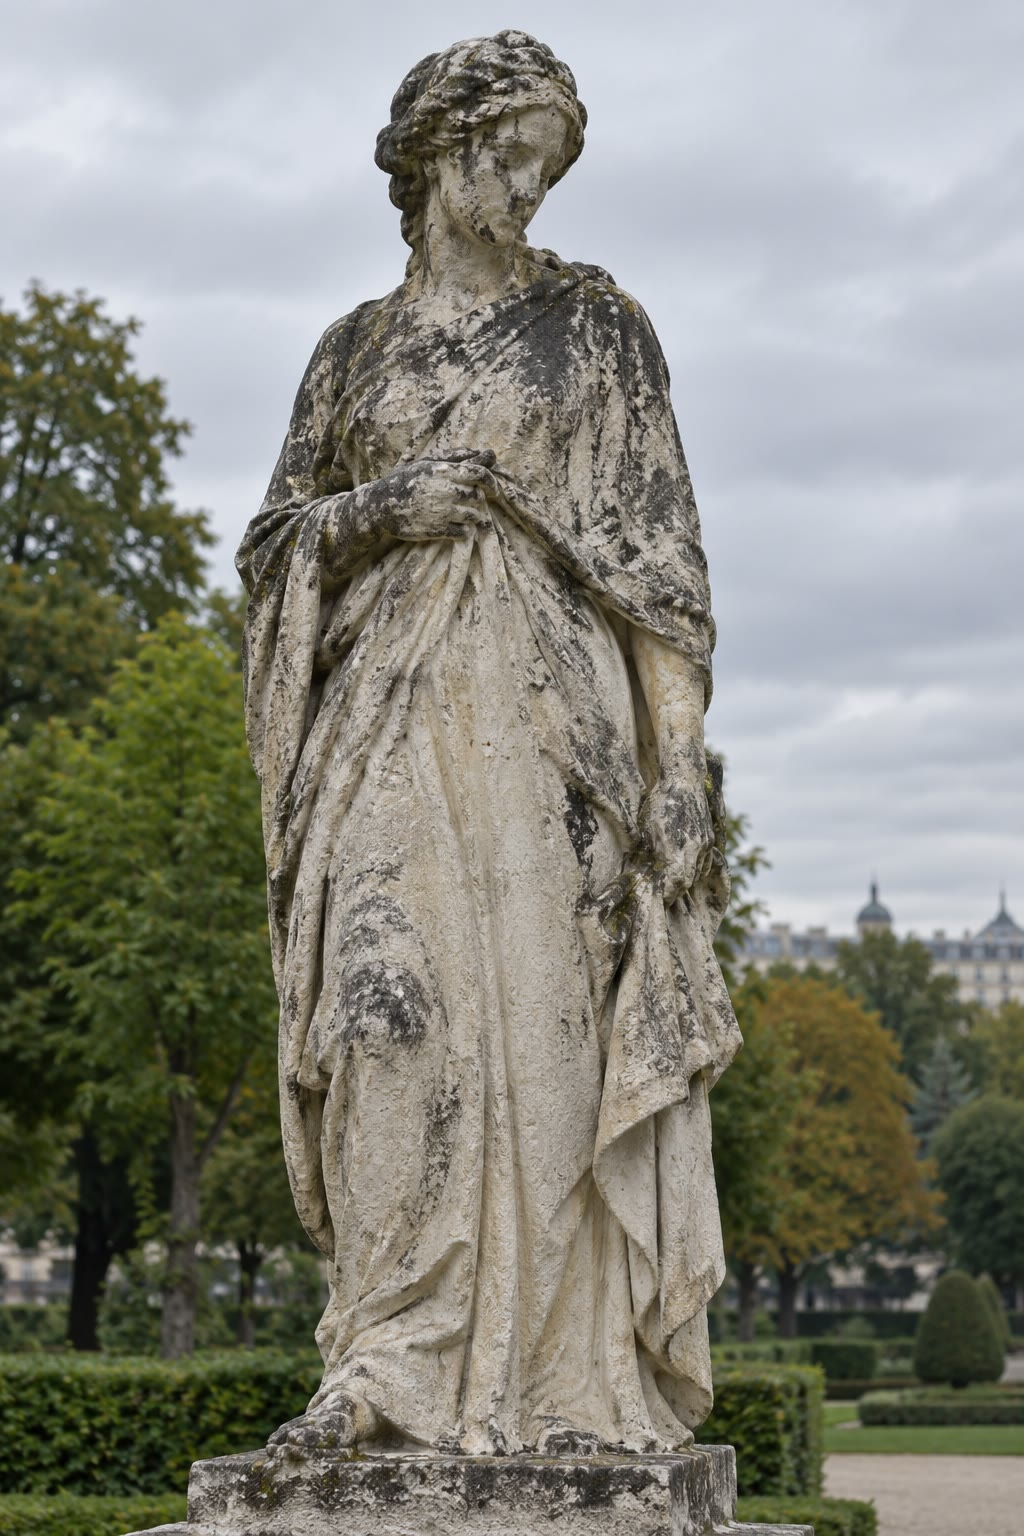
\includegraphics[width=0.42\linewidth,height=6cm,keepaspectratio]{images/book1/ai/g12-weathered-statue.jpg}

{\small Uma estátua de calcário desgastada pela chuva: uma reação que
leva séculos.}
\end{omfigure}

\section{Velocidades de consumo e de formação}

\begin{definition}[Velocidade de consumo, velocidade de formação]\label{def:g12:reaction-rates:rate}
Numa solução de volume constante, a \emph{velocidade de
consumo}\index{velocidade de consumo} de um \omterm{def:g7:chemical-reactions:reactant}{reagente} A no instante $t$ é
\[
  v_A(t) = -\frac{d[\ce{A}]}{dt},
\]
e a \emph{velocidade de formação}\index{velocidade de formacao@velocidade de formação} de um
produto P é $v_P(t) = \dfrac{d[\ce{P}]}{dt}$. As duas são positivas, em
\si{mol.L^{-1}.min^{-1}} (ou por segundo).
\end{definition}


\begin{method}[Ler uma velocidade numa tangente]\label{met:g12:reaction-rates:tangent}
\begin{enumerate}
  \item Na curva de $[\ce{A}]$ em função de $t$, trace a tangente no
        instante escolhido.
  \item Leia dois pontos bem afastados na tangente e calcule a sua
        inclinação, $\Delta[\ce{A}] / \Delta t$.
  \item A \omterm{def:g12:reaction-rates:rate}{velocidade de consumo} é o oposto dessa inclinação (para um
        produto, a própria inclinação).
\end{enumerate}
\end{method}

\begin{omfigure}
\begin{tikzpicture}
\begin{axis}[width=0.8\linewidth, height=6.4cm, xmin=0, xmax=60, ymin=0,
    ymax=11, xlabel={$t$ (\si{min})}, ylabel={$[\ce{A}]$ (\si{mmol/L})},
    axis lines*=left, ymajorgrids, xmajorgrids, grid style={gray!20},
    tick label style={font=\small}, label style={font=\small},
    legend style={font=\small, at={(0.98,0.97)}, anchor=north east,
    draw=none, fill=white}, legend cell align=left]
  \addplot[very thick, omDef] table[x=t, y=A1] {figdata/out/grade-12-reaction-rates-a.dat};
  \addplot[very thick, omThm] table[x=t, y=A2] {figdata/out/grade-12-reaction-rates-a.dat};
  \addplot[thick, dashed, omProp, restrict y to domain=0:11] table[x=t, y=tangent]
    {figdata/out/grade-12-reaction-rates-a.dat};
  \legend{$k = \qty{0.050}{min^{-1}}$, $k = \qty{0.100}{min^{-1}}$ (mais quente),
    tangente em $t = 0$}
  \addplot[densely dotted, black!60] coordinates {(0,5) (13.86,5) (13.86,0)};
  \addplot[densely dotted, black!60] coordinates {(6.93,5) (6.93,0)};
  \node[font=\small, anchor=south west] at (axis cs:14.6,5.4) {$t_{1/2} = \qty{13.9}{min}$};
  \node[font=\small, anchor=south east] at (axis cs:6.7,0.2) {\qty{6.9}{min}};
\end{axis}
\end{tikzpicture}

{\small A concentração de um \omterm{def:g7:chemical-reactions:reactant}{reagente} A em função do tempo, para a mesma
\omterm{def:g12:reaction-rates:first-order}{reação de primeira ordem} a duas temperaturas. A tangente em $t = 0$
(tracejada) dá a velocidade inicial; as linhas pontilhadas marcam as
meias-vidas.}
\end{omfigure}

\begin{example}[A velocidade inicial]\label{ex:g12:reaction-rates:initial}
Na curva azul, a tangente em $t = 0$ vai de \qty{10.0}{mmol/L} em
$t = 0$ até $0$ em $t = \qty{20}{min}$: a sua inclinação é
$-10.0/20 = \qty{-0.50}{mmol.L^{-1}.min^{-1}}$, logo a velocidade inicial
de consumo é de \qty{0.50}{mmol.L^{-1}.min^{-1}}. Depois a curva se
achata e a velocidade cai: a reação fica mais lenta à medida que A é
consumido.
\end{example}

\section{As reações de primeira ordem}

\begin{definition}[Reação de primeira ordem, constante de velocidade]\label{def:g12:reaction-rates:first-order}
Uma reação é uma \emph{reação de primeira ordem}\index{reacao de primeira ordem@reação de primeira ordem}
em relação a A se a sua \omterm{def:g12:reaction-rates:rate}{velocidade de consumo} é proporcional à
concentração de A a cada instante:
\[
  -\frac{d[\ce{A}]}{dt} = k\,[\ce{A}] .
\]
A constante positiva $k$, em \si{min^{-1}} ou \si{s^{-1}}, é a
\emph{constante de velocidade}\index{constante de velocidade}; ela
depende da temperatura.
\end{definition}

\begin{proposition}[Decaimento exponencial]\label{prop:g12:reaction-rates:exponential}
Para uma \omterm{def:g12:reaction-rates:first-order}{reação de primeira ordem} com concentração inicial
$[\ce{A}]_0$,
\[
  [\ce{A}](t) = [\ce{A}]_0\, e^{-kt} .
\]
\end{proposition}

\begin{proof}
A função $f(t) = [\ce{A}]_0 e^{-kt}$ tem derivada
$f'(t) = -k [\ce{A}]_0 e^{-kt} = -k f(t)$, logo ela satisfaz a equação
de velocidade, e $f(0) = [\ce{A}]_0$. Que ela seja a única função assim
é admitido aqui (isso é demonstrado em matemática, para as equações
$y' = ay$).
\end{proof}

\begin{method}[Testar a primeira ordem]\label{met:g12:reaction-rates:test}
\begin{enumerate}
  \item A partir das medidas, calcule $\ln [\ce{A}]$ (ou $\ln A$ para
        uma \omterm{def:g11:absorbance:absorbance}{absorbância} proporcional a $[\ce{A}]$) em cada instante.
  \item Trace $\ln[\ce{A}]$ em função de $t$: como
        $\ln[\ce{A}] = \ln[\ce{A}]_0 - kt$, os pontos ficam numa reta se
        e somente se a reação é de primeira ordem.
  \item A inclinação da reta é $-k$.
\end{enumerate}
\end{method}

\section{A meia-vida}

\begin{definition}[Meia-vida]\label{def:g12:reaction-rates:half-life}
A \emph{meia-vida}\index{meia-vida} $t_{1/2}$ de uma reação é o tempo
necessário para que a concentração do \omterm{def:g10:reaction-progress-table:limiting}{reagente limitante} caia à metade
do seu valor inicial.
\end{definition}

\begin{proposition}[A meia-vida de uma reação de primeira ordem]\label{prop:g12:reaction-rates:half-life}
Para uma \omterm{def:g12:reaction-rates:first-order}{reação de primeira ordem},
\[
  t_{1/2} = \frac{\ln 2}{k},
\]
qualquer que seja a concentração inicial; depois de $n$ meias-vidas, a
concentração está dividida por $2^n$.
\end{proposition}

\begin{proof}
$[\ce{A}]_0 e^{-k t_{1/2}} = [\ce{A}]_0 / 2$ dá $e^{-k t_{1/2}} = 1/2$,
logo $k t_{1/2} = \ln 2$. Cada nova \omterm{def:g12:reaction-rates:half-life}{meia-vida} multiplica de novo a
concentração por $e^{-k t_{1/2}} = 1/2$.
\end{proof}


\begin{example}[Ler as meias-vidas]\label{ex:g12:reaction-rates:half-lives}
Para $k = \qty{0.050}{min^{-1}}$, $t_{1/2} = 0.693 / 0.050 =
\qty{13.9}{min}$: a concentração cai de 10.0 para 5.0, depois 2.5, depois
\qty{1.25}{mmol/L} em 13.9, 27.7 e \qty{41.6}{min}. O experimento mais
quente, com um $k$ duas vezes maior, tem metade da \omterm{def:g12:reaction-rates:half-life}{meia-vida},
\qty{6.9}{min}, como mostra a figura.
\end{example}

\begin{remark}[Meias-vidas em outros lugares]\label{rem:g12:reaction-rates:radioactive}
A mesma palavra é usada em física para os \omterm{def:g9:inside-the-atom:nucleus}{núcleos} radioativos, cujo
número diminui da mesma maneira exponencial: um decaimento radioativo se
comporta como uma \omterm{def:g12:reaction-rates:first-order}{reação de primeira ordem}. O livro de física trata
disso.
\end{remark}

\begin{omfigure}
\begin{minipage}{0.49\linewidth}
\begin{tikzpicture}
\begin{axis}[width=\linewidth, height=5.4cm, xmin=0, xmax=26, ymin=0,
    ymax=0.85, xlabel={$t$ (\si{min})}, ylabel={absorbância $A$},
    axis lines*=left, ymajorgrids, grid style={gray!20},
    tick label style={font=\scriptsize}, label style={font=\small}]
  \addplot[only marks, mark=*, mark size=1.8pt, omDef] table[x=t, y=A]
    {figdata/out/grade-12-reaction-rates-b.dat};
  \addplot[thick, omProp, domain=0:26, samples=60] {0.8*exp(-0.11552*x)};
\end{axis}
\end{tikzpicture}
\end{minipage}\hfill
\begin{minipage}{0.49\linewidth}
\begin{tikzpicture}
\begin{axis}[width=\linewidth, height=5.4cm, xmin=0, xmax=26, ymin=-3.4,
    ymax=0, xlabel={$t$ (\si{min})}, ylabel={$\ln A$}, axis lines*=left,
    ymajorgrids, grid style={gray!20}, tick label style={font=\scriptsize},
    label style={font=\small}]
  \addplot[only marks, mark=*, mark size=1.8pt, omDef] table[x=t, y=lnA]
    {figdata/out/grade-12-reaction-rates-b.dat};
  \addplot[thick, omProp, domain=0:26] {-0.2231-0.11552*x};
\end{axis}
\end{tikzpicture}
\end{minipage}

{\small O descoramento do cristal violeta numa \omterm{def:g9:acids-bases-ph:acidic}{solução básica} (dados do
problema de fim de semana). À esquerda: a \omterm{def:g11:absorbance:absorbance}{absorbância} cai seguindo uma
exponencial. À direita: $\ln A$ em função de $t$ é uma reta de
inclinação $-\qty{0.116}{min^{-1}}$: a reação é de primeira ordem em
relação ao corante.}
\end{omfigure}

\section{Exercícios}

\begin{exercise}[$\star$]\label{exo:g12:reaction-rates:1}
Dê o nome do \omterm{def:g12:reaction-rates:kinetic-factor}{fator cinético} que atua em cada caso: uma geladeira
conserva os alimentos; o açúcar em pó \omterm{def:g2:mixing-and-dissolving:dissolve}{se dissolve} mais depressa que um
torrão; um ácido mais concentrado ataca o zinco mais depressa; uma maçã
cortada escurece mais depressa no verão.
\end{exercise}

\begin{exercise}[$\star$]\label{exo:g12:reaction-rates:2}
Leia na figura de $[\ce{A}]$ em função do tempo a \omterm{def:g12:reaction-rates:half-life}{meia-vida} de cada
experimento. Quanto vale $[\ce{A}]$ na curva azul depois de duas
meias-vidas?
\end{exercise}

\begin{exercise}[$\star$]\label{exo:g12:reaction-rates:3}
Uma tangente à curva de um produto, traçada em $t = \qty{5}{min}$, passa
por $(0, \qty{1.0}{mmol/L})$ e $(\qty{10}{min}, \qty{5.0}{mmol/L})$.
Qual é a \omterm{def:g12:reaction-rates:rate}{velocidade de formação} do produto em \qty{5}{min}?
\end{exercise}

\begin{exercise}[$\star$]\label{exo:g12:reaction-rates:4}
Por que uma amostra é despejada em água gelada antes de ser titulada?
Por que o instante da amostra deve ser anotado quando ela é despejada, e
não quando ela é titulada?
\end{exercise}

\begin{exercise}[$\star$]\label{exo:g12:reaction-rates:5}
Uma \omterm{def:g12:reaction-rates:first-order}{reação de primeira ordem} tem uma \omterm{def:g12:reaction-rates:half-life}{meia-vida} de \qty{10}{min}. Que
fração do \omterm{def:g7:chemical-reactions:reactant}{reagente} resta depois de \qty{30}{min}? E depois de
\qty{1}{h}?
\end{exercise}

\begin{exercise}[$\star\star$]\label{exo:g12:reaction-rates:6}
Concentrações de um \omterm{def:g7:chemical-reactions:reactant}{reagente}, em \si{mmol/L}: 8.00 em \qty{0}{min}, 5.66
em \qty{5}{min}, 4.00 em \qty{10}{min}, 2.83 em \qty{15}{min}, 2.00 em
\qty{20}{min}. Calcule $\ln[\ce{A}]$ em cada instante e mostre que a
reação é de primeira ordem. Encontre $k$ e a \omterm{def:g12:reaction-rates:half-life}{meia-vida}.
\end{exercise}

\begin{exercise}[$\star\star$]\label{exo:g12:reaction-rates:7}
Uma \omterm{def:g12:reaction-rates:first-order}{reação de primeira ordem} tem $t_{1/2} = \qty{25}{s}$. Calcule $k$.
\end{exercise}

\begin{exercise}[$\star\star$]\label{exo:g12:reaction-rates:8}
Para $[\ce{A}]_0 = \qty{0.100}{mol/L}$ e $k = \qty{0.020}{min^{-1}}$,
calcule $[\ce{A}]$ depois de 10, 30 e \qty{100}{min}.
\end{exercise}

\begin{exercise}[$\star\star$]\label{exo:g12:reaction-rates:9}
Na figura de $[\ce{A}]$ em função do tempo, estime a inclinação da curva
azul em $t = \qty{13.9}{min}$ (trace uma tangente), e compare-a com
$-k[\ce{A}]$ nesse instante.
\end{exercise}

\begin{exercise}[$\star\star$]\label{exo:g12:reaction-rates:10}
O iodo \ce{I2}, marrom, se forma lentamente numa solução incolor. A
\omterm{def:g11:absorbance:absorbance}{absorbância} sobe de 0 em direção a 0.60. Explique por que a \omterm{def:g11:absorbance:absorbance}{absorbância}
pode ser usada para acompanhar $[\ce{I2}]$, e como a \omterm{def:g12:reaction-rates:rate}{velocidade de
formação} num dado instante é lida na curva de $A$ em função de $t$.
\end{exercise}

\begin{exercise}[$\star\star$]\label{exo:g12:reaction-rates:11}
Dois experimentos da mesma reação começam com $[\ce{A}]_0 = 10$ e
\qty{20}{mmol/L}. Se a reação é de primeira ordem, compare as suas
velocidades iniciais e as suas meias-vidas.
\end{exercise}

\begin{exercise}[$\star\star\star$]\label{exo:g12:reaction-rates:12}
Quantas meias-vidas uma \omterm{def:g12:reaction-rates:first-order}{reação de primeira ordem} leva para chegar a
\qty{1}{\percent} do seu \omterm{def:g7:chemical-reactions:reactant}{reagente}? E a \qty{0.1}{\percent}? Dê a fórmula
geral do tempo necessário para cair a uma fração $f$.
\end{exercise}

\begin{exercise}[$\star\star\star$]\label{exo:g12:reaction-rates:13}
Uma reação tem $k = \qty{0.050}{min^{-1}}$ a \qty{20}{\celsius} e
$k = \qty{0.100}{min^{-1}}$ a \qty{30}{\celsius}. Quanto tempo ela leva
para consumir \qty{90}{\percent} do \omterm{def:g7:chemical-reactions:reactant}{reagente} a cada temperatura? Uma
regra prática comum diz que a velocidade dobra a cada
\qty{10}{\celsius}: esta reação a segue?
\end{exercise}

\begin{exercise}[$\star\star\star$]\label{exo:g12:reaction-rates:14}
Interrompe-se a reação numa amostra despejando \qty{5.0}{mL} dela em
\qty{45}{mL} de água gelada. Dê duas razões pelas quais a reação fica
muito mais lenta. Se a reação é de primeira ordem em relação a cada um
de dois \omterm{def:g7:chemical-reactions:reactant}{reagentes}, por que fator a \omterm{def:g10:concentration-and-dilution:dilution}{diluição} sozinha divide a velocidade?
\end{exercise}

\begin{exercise}[$\star\star\star$]\label{exo:g12:reaction-rates:15}
Mostre, derivando, que a \omterm{def:g12:reaction-rates:rate}{velocidade de consumo} de uma \omterm{def:g12:reaction-rates:first-order}{reação de
primeira ordem} é ela própria uma função exponencial do tempo,
$v(t) = k[\ce{A}]_0 e^{-kt}$. Qual é a velocidade inicial? Depois de
quanto tempo a velocidade é a metade da velocidade inicial?
\end{exercise}

\section{Problema: o corante que desbota}

\begin{problem}[{Problema de fim de semana --- o cristal violeta descorado
pelos íons hidróxido: quanto tempo até a cor quase desaparecer?}]
\label{pb:g12:reaction-rates:1}
O corante violeta chamado cristal violeta reage com os \omterm{def:g9:ions:ion}{íons} hidróxido e
dá um produto incolor. Com um grande excesso de hidróxido, a velocidade
só depende da concentração do corante. A \omterm{def:g11:absorbance:absorbance}{absorbância} da solução é
registrada no comprimento de onda em que o corante absorve mais:
\begin{center}
\small
\begin{tabular}{l*{10}{c}}
\hline
$t$ (\si{min}) & 0 & 2 & 4 & 6 & 8 & 10 & 12 & 15 & 20 & 25 \\
$A$ & 0.800 & 0.639 & 0.501 & 0.402 & 0.315 & 0.255 & 0.199 & 0.143 &
0.078 & 0.046 \\
\hline
\end{tabular}
\end{center}

\medskip
\noindent\textbf{Parte I --- \omterm{def:g11:absorbance:absorbance}{Absorbância} e concentração.}
\begin{enumerate}
  \item Por que a \omterm{def:g11:absorbance:absorbance}{absorbância} é proporcional à concentração do corante?
        Que condição a solução deve satisfazer?
  \item Por que o produto, incolor, não é visto nesse comprimento de
        onda?
  \item Por que o hidróxido é usado em grande excesso?
  \item O que se leria no espectrofotômetro no fim da reação?
\end{enumerate}

\medskip
\noindent\textbf{Parte II --- É de primeira ordem?}
\begin{enumerate}[resume]
  \item Leia a \omterm{def:g12:reaction-rates:half-life}{meia-vida} diretamente na tabela.
  \item Verifique que ela é a mesma de $t = 6$ a $t = 12$ min.
  \item Calcule $\ln A$ para cada instante.
  \item Trace $\ln A$ em função de $t$ (ou use a figura do capítulo). O
        que você observa? Conclua.
  \item Calcule a inclinação a partir dos pontos em 0 e \qty{20}{min}.
\end{enumerate}

\medskip
\noindent\textbf{Parte III --- A \omterm{def:g12:reaction-rates:first-order}{constante de velocidade}.}
\begin{enumerate}[resume]
  \item Deduza $k$.
  \item Calcule a \omterm{def:g12:reaction-rates:half-life}{meia-vida} a partir de $k$, e compare com a questão 5.
  \item Calcule a velocidade inicial de consumo do corante, expressa
        como uma velocidade de diminuição da \omterm{def:g11:absorbance:absorbance}{absorbância}.
  \item Qual seria a \omterm{def:g12:reaction-rates:half-life}{meia-vida} se a \omterm{def:g11:absorbance:absorbance}{absorbância} inicial fosse 0.400?
\end{enumerate}

\medskip
\noindent\textbf{Parte IV --- Previsão.}
\begin{enumerate}[resume]
  \item Preveja a \omterm{def:g11:absorbance:absorbance}{absorbância} em \qty{30}{min}.
  \item Em que instante a \omterm{def:g11:absorbance:absorbance}{absorbância} cai a 0.008, \qty{1}{\percent} do
        seu valor inicial?
  \item Quantas meias-vidas são isso?
  \item O olho deixa de ver a cor abaixo de cerca de $A = 0.010$. Quando
        a solução parece incolor?
  \item O experimento é repetido \qty{10}{\celsius} mais quente, e a
        \omterm{def:g12:reaction-rates:half-life}{meia-vida} passa a ser \qty{3.0}{min}. Quando se chega a
        \qty{1}{\percent}?
  \item Dê a resposta final: quantas meias-vidas a cor leva para cair a
        \qty{1}{\percent} do seu valor inicial, e quantos minutos são
        isso aqui?
\end{enumerate}
\end{problem}
